% ----------------------------------------------------------------------^
% Copyright (C) 2004, 2005, 2006, 2007, 2008 Giorgio Calderone
% (mailto: <gcalderone@ifc.inaf.it>)
% 
% This file is part of MCS.
% 
% MCS is free software; you can redistribute it and/or modify
% it under the terms of the GNU General Public License as published by
% the Free Software Foundation; either version 2 of the License, or
% (at your option) any later version.
% 
% MCS is distributed in the hope that it will be useful,
% but WITHOUT ANY WARRANTY; without even the implied warranty of
% MERCHANTABILITY or FITNESS FOR A PARTICULAR PURPOSE.  See the
% GNU General Public License for more details.
% 
% You should have received a copy of the GNU General Public License
% along with MCS; if not, write to the Free Software
% Foundation, Inc., 51 Franklin St, Fifth Floor, Boston, MA  02110-1301  USA
% 
% ----------------------------------------------------------------------$

% http://infa.abo.fi/~chakie/zombie/docs/zombie/c14.html

\documentclass[12pt,titlepage]{book}
\usepackage[english]{babel}
\usepackage{graphicx}
\usepackage[lineno1,leftno]{lgrind}


\textheight 22cm
\textwidth 16.5cm
\topmargin 0cm
\oddsidemargin -0.5cm
\evensidemargin -0.5cm
\sloppy

\newcommand{\mcs}{\textbf{MCS} }

\def\ver{Ver. 0.2.2}

\begin{document}
\frontmatter


\title{
%
\sffamily \textbf{MCS \\ My Customizable Server}
%
\thanks{http://spora.ifc.inaf.it/mcs}
%
\vspace{3cm}
%\includegraphics[width=10cm,keepaspectratio]{./includes/sport_logo_gray} \\
\vspace{2.5cm}
%
\centerline{\rule{\textwidth}{0.4pt}}
%
}
\bigskip
\author{
  \sc{Giorgio Calderone}
  \footnote{Giorgio Calderone $<$gcalderone@ifc.inaf.it$>$}  \\
  \sc{IFC - INAF Palermo, Italy} \\ \\
  \sc{Luciano Nicastro}
  \footnote{Luciano Nicastro $<$nicastro@iasfbo.inaf.it$>$} \\
  \sc{IASF - INAF Bologna, Italy}
 }

\date{14 May 2006 \\ \ver \\ \centerline{\rule{\textwidth}{0.4pt}}}
%
\maketitle

\tableofcontents
\mainmatter

\chapter{Introduction}

Today's information services can be separated in two classes: those in
which information produced are destined to humans, and those in which
information produced are destined to other software applications. In
the former case there is a quite standardized way to develop such a
information service, essentially based upon a web server, a database
server, a scripting language and the HTML language. In the latter case
there is no such standardization, because of the wide landscape of
software and solutions given to the developer, and also to the
different kind of problems users have to deal with.

\bigskip

\noindent The \mcs project propose a unified model to standardize the
developing process of information services, without worrying about the
low level networking, threading and database code.

\bigskip

\noindent So MCS and its protocol are to software applications, what a
web server and HTTP are for the WWW: a simple way to access data. In
this comparison customizing the MCS server is like writing a web page.

\bigskip

\noindent The \mcs project was developed at IFC-INAF (Palermo, Italy)
by Giorgio Calderone and Luciano Nicastro.

\section{What is MCS ?}
\label{sec-whatismcs}
\mcs is a set of C++ high level, easy to use, classes aimed at
implementing an application server, that is an application that
provides a service over the network. Its main features are the
possibility to customize the server behaviour through the derivation
of some classes, and the usage of a well defined communication
protocol (the \mcs protocol).

\bigskip

\noindent With \mcs you can easily implement custom services on top of
which different users can perform requests to a common database
through several tools obtaining different types of data, depending on
the tool used and the user permissions. The \mcs protocol and software
tools let user’s applications obtain data in a well defined binary
fashion or plain text, so that they are ready to be further processed.

\noindent Informations servers based upon \mcs can be implemented
without worrying about TCP connections, multi-threading, database code
and so on. You only need to focus on the main problem, and write just
the code needed to realize the tasks that characterize the service to
your needs. Some of other features of \mcs are:

\begin{itemize}
\item easy to configure;
\item authentication and grant support;
\item database access;
\item base commands set, support to create new customized commands;
\item accessibility from other languages such as C, Fortran, IDL, PHP,
ecc...;
\item logging facility, ecc...;
\end{itemize}

\bigskip

\noindent Furthermore, many \mcs's classes such as \verb|Thread|,
\verb|Socket|, \verb|Query|, etc..., are general purpose so that you
can use them also in non-server applications. While these are high
level classes, and so very easy to use, they're not intended to be an
exhaustive framework to work with threads, sockets, and so on (for
these tasks there are already a number of packets around, such as
CommonC++, wvStreams, etc...). We think that if your application needs
such a complete control over these subjects you should spend your time
to learn and use directly the system's library.


\section{License issues}
\label{sec-license}
\mcs is distributed free of charge and according to the GNU General
Public License. This means that you may copy this software and
distribute it free of charge, as well as modify it provided that you
retain this note and mention the authors name. The GNU General Public
License comes with this package in a file named COPYING, for more
information about this license visit \verb|www.gnu.org|.



\section{Some simple examples}
\label{sec-somesimpleexamples}
This section is aimed to give a first sight at the code you should
deal with if you decide to write an \mcs based application.

\bigskip

\noindent In the first example we'll build a simple application server
without any customization, with all base commands available (see
Sect. \ref{sec:commands}). These commands gives you the following
possibilities: authentication support, database access, file download
and upload, access to external programs. All these facilities are
immediately available, without writing a single line of code for
them. Each facility can be also disabled, using an external
configuration file. The code is shown in Fig. \ref{source:simplest},
it is called ``simplest'' because it is the simplest server you can
build with \mcs.

\lagrind[hbtp]{includes/simplest.cc.tex}{Source of simplest.cc}
{source:simplest}

\bigskip

\noindent In the second example, called ``echosrv'', whose code is
shown in Fig. \ref{source:echosrv}, we'll build the classical echo
server, that is a server which reply with the same string you send as
command. Here we can see a little customization of the
\verb|UserThread| class, in the line 8 and 9 of the code. All other
lines are standard code which is to be used for any customized
application. All facilities mentioned above are still present there.

\lagrind[hbtp]{includes/echosrv.cc.tex}{Source of echosrv.cc}{source:echosrv}


\section{About this document}
\label{sec:aboutthisdocument}

This document describes the technical aspects of the \mcs software,
and show how a customized application server can be built using
\mcs. This document presumes that the reader is familiar with C++ and
programming under Linux.

\bigskip

\noindent This document is work in progress, so you should always look
for the last version because some fundamental parts are being
rewritten or will be available in the next future. If you find any
errors we'd appreciate if you could send us an email\footnote{Giorgio
Calderone $<$gcalderone@ifc.inaf.it$>$, Luciano Nicastro
$<$nicastro@iasfbo.inaf.it$>$}. Thanks in advance.

\bigskip

\noindent The \mcs documentation is divided in several chapters so
that you can read only the information you need:
\begin{itemize}
\item \textbf{User's manual}: gives an overview of an \mcs based
  system and focus on how to acces an \mcs service as a client, it
  also explain in details all base commands;

\item \textbf{Interface to MCS}: describes all available interface to
  connect to \mcs through other languages;

\item \textbf{Developer's manual}: intended for users who wants to
  implement information services using \mcs;

%\item \textbf{Administrator manual}: intended for users who wants to
%  build or maintain a \mcs based application;

\item \textbf{Examples}: examples that shows how to implement
  information services with \mcs;

\item \textbf{libmcs reference}\footnote{available only in HTML format
  at: http://spora.ifc.inaf.it/mcs}: technical description of the \mcs
  library implementation;
\end{itemize}



%---------------------------------------------------------------------
\chapter{User's manual}
\label{chap:usermanual}

\section{Installing MCS}
\label{sec:installing}
The \mcs software is distributed in a \verb|tar.gz| package, to unpack
it simply issue the command:

\bigskip

\verb|tar xvzf mcs-x.y.z.tar.gz|

\bigskip

\noindent where x, y, z are the version number. A directory named
\verb|mcs-x.y.z| will be created containing all sources code as well
as the documentation and the scripts needed to install \mcs. Before
installing \mcs you should check that all mandatory dependencies are
satisfied (see Sect. \ref{ssec:dependencies}), then you must follow a
three step procedure: configure, compile and install.

\subsubsection{Configure}
\label{sssec:configuremcs}
Configuring \mcs means check your system for compatibilities, search
for include files and libraries, and finally produce all necessary
makefiles needed to compile \mcs. This is done automatically by the
\verb|configure| script distributed with \mcs. Typically you can use
this script without any option, as follows:

\bigskip

\verb|./configure|

\bigskip

\noindent Anyway \verb|configure| has a lot of options and switches
(type \verb|configure --help| for a list) to customize the compilation
step. Some of these options are specific to \mcs:

\begin{itemize}
\item \verb|--prefix=PATH| \\ The directory under which all include files,
  libraries and other files relative to \mcs will be stored, if this
  option is not used \verb|usr/local| is used.

\item \verb|--with-pcre=PATH| \\ if the PCRE package is not installed
  in a standard location (typically \verb|/usr/local|) you can provide
  the correct path with this option.

\item \verb|--enable-debug, --disable-debug| \\ if enabled will add
  the "-g" and "-O0" flags to the compiler command line, these are
  needed to include debugging information in the library and to
  discard any optimization. By default this option is disabled.


\item \verb|--enable-mysql, --disable-mysql| \\ enable or disable
  the compilation of MySQL facilities. By default this option is
  enabled.


\item \verb|--enable-cfitsio, --disable-cfitsio| \\ enable or disable
  the compilation of CFITSIO facilities (Query::Fits2Table and
  Query::Result2Fits methods). By default this option is enabled.

\item \verb|--with-cfitsio=PATH| \\ if the CFITSIO package is not
  installed in a standard location (typically
  \verb|/usr/local/cfitsio|) you can provide the correct path with
  this option.


\item \verb|--enable-idl, --disable-idl| \\ enable or disable the
  compilation of the IDL to \mcs interface. By default this option is
  enabled.

\item \verb|--with-idl=PATH| \\ if the IDL package is not installed in
  a standard location (typically /usr/local/rsi/idl) you can provide the
  correct path with this option.


\item \verb|--enable-php| \\ enable or disable the compilation of the
  PHP to \mcs interface. By default this option is enabled.
\end{itemize}

\noindent There are a lot of other options and switches, for further
documentation see the \verb|INSTALL| file.



\subsubsection{Compile}
\label{sssec:compilemcs}
To compile \mcs simply issue the command:

\bigskip

\verb|make|

\bigskip

\noindent If you got error while compiling check
Sect. \ref{sssec:configuremcs} and the \verb|INSTALL| file.


\subsubsection{Install}
\label{sssec:installmcs}
If \mcs has been correctly compiled you can install with the command:

\bigskip

\verb|make install|

\bigskip

\noindent If your account doesn't have the permission to write in the
path where should be installed you will get an error. In this case you
should login as ``root'' and retry.



\subsection{Dependencies}
\label{ssec:dependencies}

\noindent \mcs depends on a number of other software packages that
must be installed on your system before installing \mcs:
\begin{itemize}
\item PCRE (ver. $>= 6.4$, \verb|www.pcre.org|, mandatory);
\item MySQL (ver. $>= 5.0.18$, \verb|www.mysql.org|, optional) used to
  connect to database, and to handle client authentications and
  grants;
\item LIBXML2 (ver. $>= 2.6.23$, \verb|xmlsoft.org|, optional) used to
  read and write data in the VOTable
  \footnote{www.ivoa.net/Documents/latest/VOT.html} format;
\item CFITSIO (ver. $>= 2.510$ ,
  \verb|heasarc.gsfc.nasa.gov/lheasoft/fitsio/fitsio.html|, optional)
  used to read and write data in the FITSIO format;
\item IDL (ver. $>= 5.6$, \verb|rsinc.com/idl|, optional) used to
  implement the IDL to \mcs interface;
\item PHP (ver. $>= 5.0.5$, \verb|www.php.net|, optional) used to
  implement the PHP to \mcs interface. Note that you need the complete
  source code (also called ``development package''),
\end{itemize}

\noindent Mandatory packages (actually only PCRE) are included in the
\verb|contrib| directory. If these packages aren't present in the
system they will be automatically configured, compiled and installed
in the same directory as \mcs (default \verb|/usr/local|).

\bigskip

\noindent If the optional packages aren't present in the system the
corresponding facility will be disabled.


\section{Architecture of a MCS based system}
\label{sec:architecture}
A \mcs based system has four main components (see
Fig. \ref{fig:maincomponents}):

%
\begin{figure}[hbtp]
\begin{center}
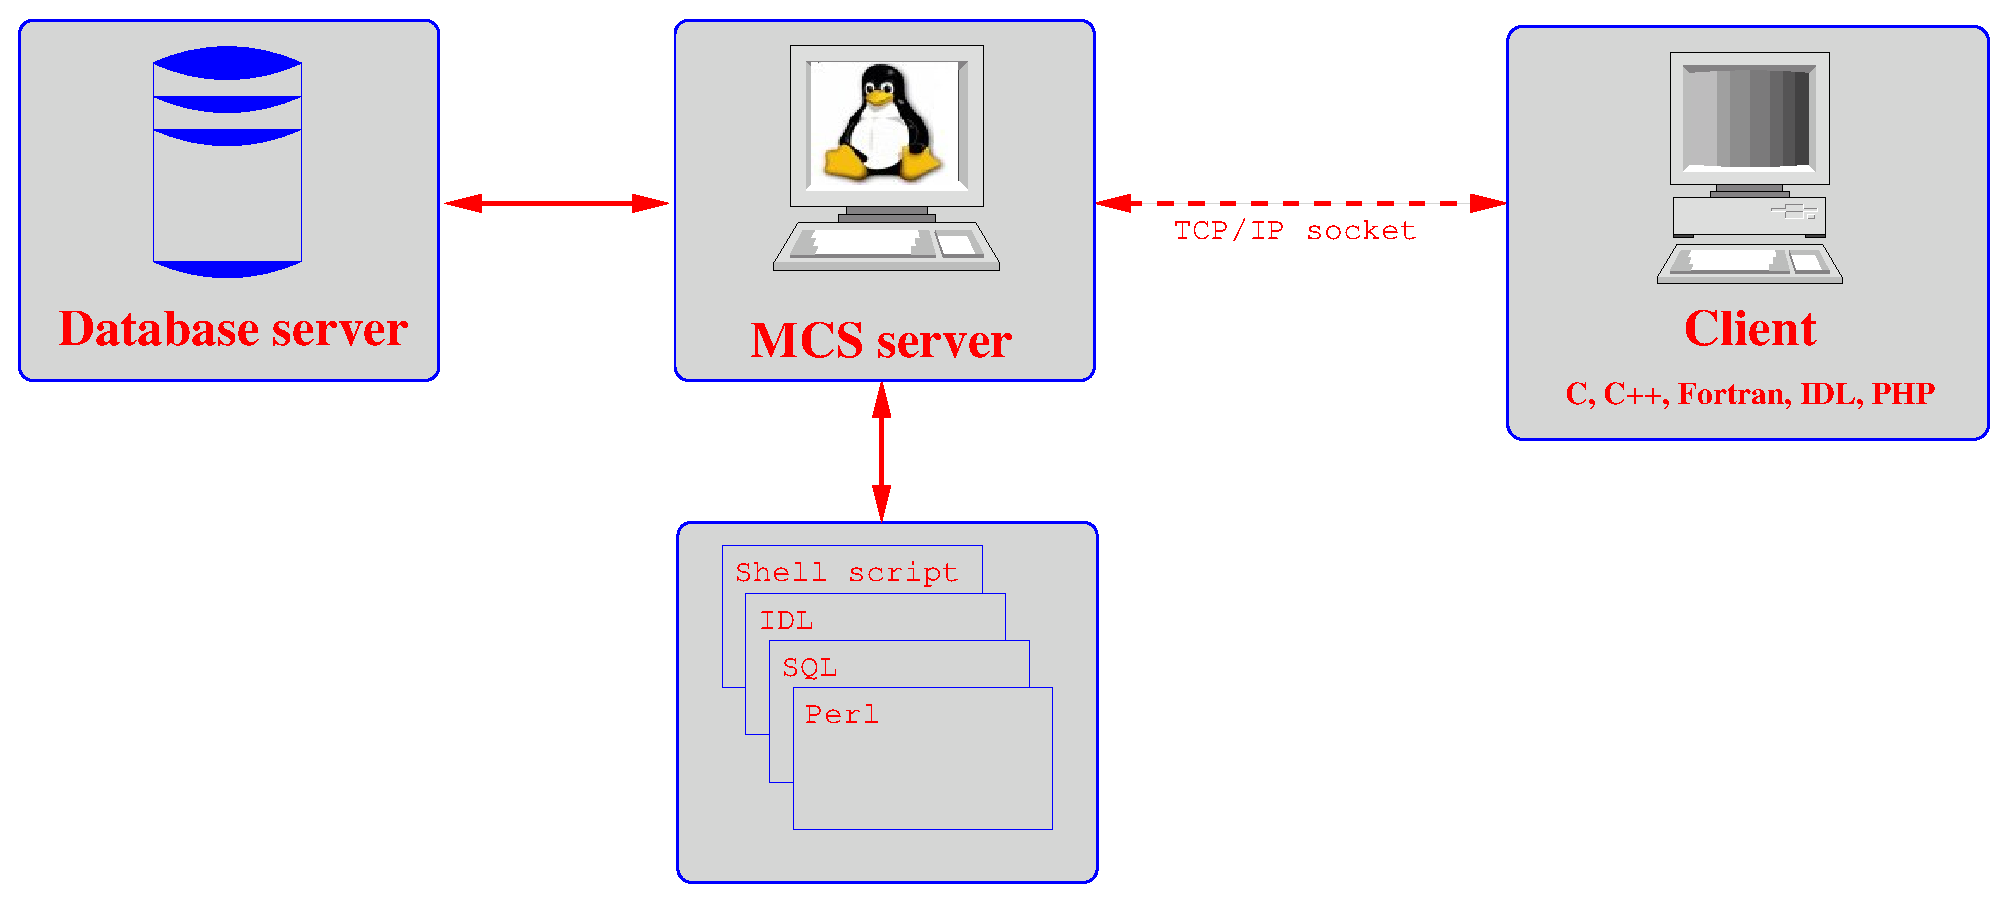
\includegraphics[width=14cm,keepaspectratio]{includes/diaggen}
\end{center}
\caption{Main component of a MCS based system}
\label{fig:maincomponents}
\end{figure}
%

\subsubsection{Database server}
The database server is used to handle clients authentication, store
all application specific data, and everything is necessary to the
application itself. This server isn't accessible directly from
clients, but only through the application server. Actually the only
supported database server is MySQL \footnote{http://www.mysql.org},
but in the future other database may become accessible through \mcs.

\subsubsection{Application server (based upon MCS)}
The application server is the core of the information system. It
implement the client/server model: a client open a TCP socket towards
the host running \mcs and sends a request through this, then the
server compute an answer, eventually access the database or execute
some external programs, and sends the answer back to the client. The
behaviour of the \mcs server can be customized deriving some classes
(see Chap. \ref{chap:developer}).

\subsubsection{External programs}
External programs are software written in any language, which interact
with the application server via command line and the stadard output.
The support to this programs were added to easily integrate already
existent applications with \mcs.


\subsubsection{Clients}
Clients are programs which access the \mcs service over the
network. Such programs can be written in any language and run on any
platform, provided that they implement the \mcs protocol. Interfaces
that implements the \mcs protocol are provided by the \mcs library for
the following languages on the Linux platform: C, C++, Fortran, IDL,
PHP. Support for other languages (such as Java and Perl) and the
Windows platform will be available soon.


\section{The MCS server}
\label{sec:themcsserver}
The \mcs server is an application server, that is an application that
waits on a TCP port until some client connect. Once a client connects
the server provide an information service, that is the possibility of
requesting informations to the server. Data are trasmitted using the
\mcs protocol, which must be implemented by the clients. This protocol
is flexible enough to trasmit binary data and files, but also to let a
client access the service offered by \mcs froma simple telnet client
(using the ``text mode'', see TODO). Due to the flexibility of the
protocol, \mcs is the natural solution to implement communication
between different software tools running on different hosts, through
the network. So \mcs can also perform IPC (Inter Process
Communication).

\subsection{Customize the MCS server}
\label{ssec:customizemcs}
One of the main feature of \mcs is the possibility to be customized,
adapting the server behaviour to specific tasks. \mcs can be
customized in several ways:

\begin{itemize}
\item adding external programs, either real external applications or
  batch lists of \mcs commands;
\item adding SQL programs, to be executed on the database server;
\item adding customized commands, deriving the \verb|UserThread|
  class;
\item modifying the behaviour of the local thread, deriving the
  \verb|LocalThread| class;
\end{itemize}

\noindent We'll explain in detail how to customize the \mcs server in
Chap. \ref{chap:developer}.


\subsection{Comparison with a ``shell''}
Using an \mcs server is very similar to the usage of a classic unix
shell, that is a prompt on which users can execute commands in their
own environment, and wait for the output before a new command is
issued. It is therefore possible to make a comparison between the
``components'' of a shell, and the ones from a \mcs connection (see
Tab. \ref{paragoneshell}). The concepts listed herein will be
described in details later.

%
\begin{table}[hbtp] \begin{center}
    \bigskip
    \begin{tabular}{|l|l|}
      \hline \textbf{Unix shell} & \textbf{MCS server} \\ \hline
      \verb|stdin| e \verb|stdout| & bidirectional TCP socket \\
      system account & MySQL account \\ internal commands & base
      commands \\ programs, shell scripts & external programs
      (\verb|EXEC| command) \\ home directory & work directory \\
      \hline
    \end{tabular}
    \caption{``shell'' comparison}\label{paragoneshell}
\end{center} \end{table}
%

\subsection{Temporal sequence of events during a connection}
In this section we'll explain the temporal sequence of events during a
\mcs session, using Fig. \ref{flow}.
%
\begin{figure}[hbtp]
\begin{center}
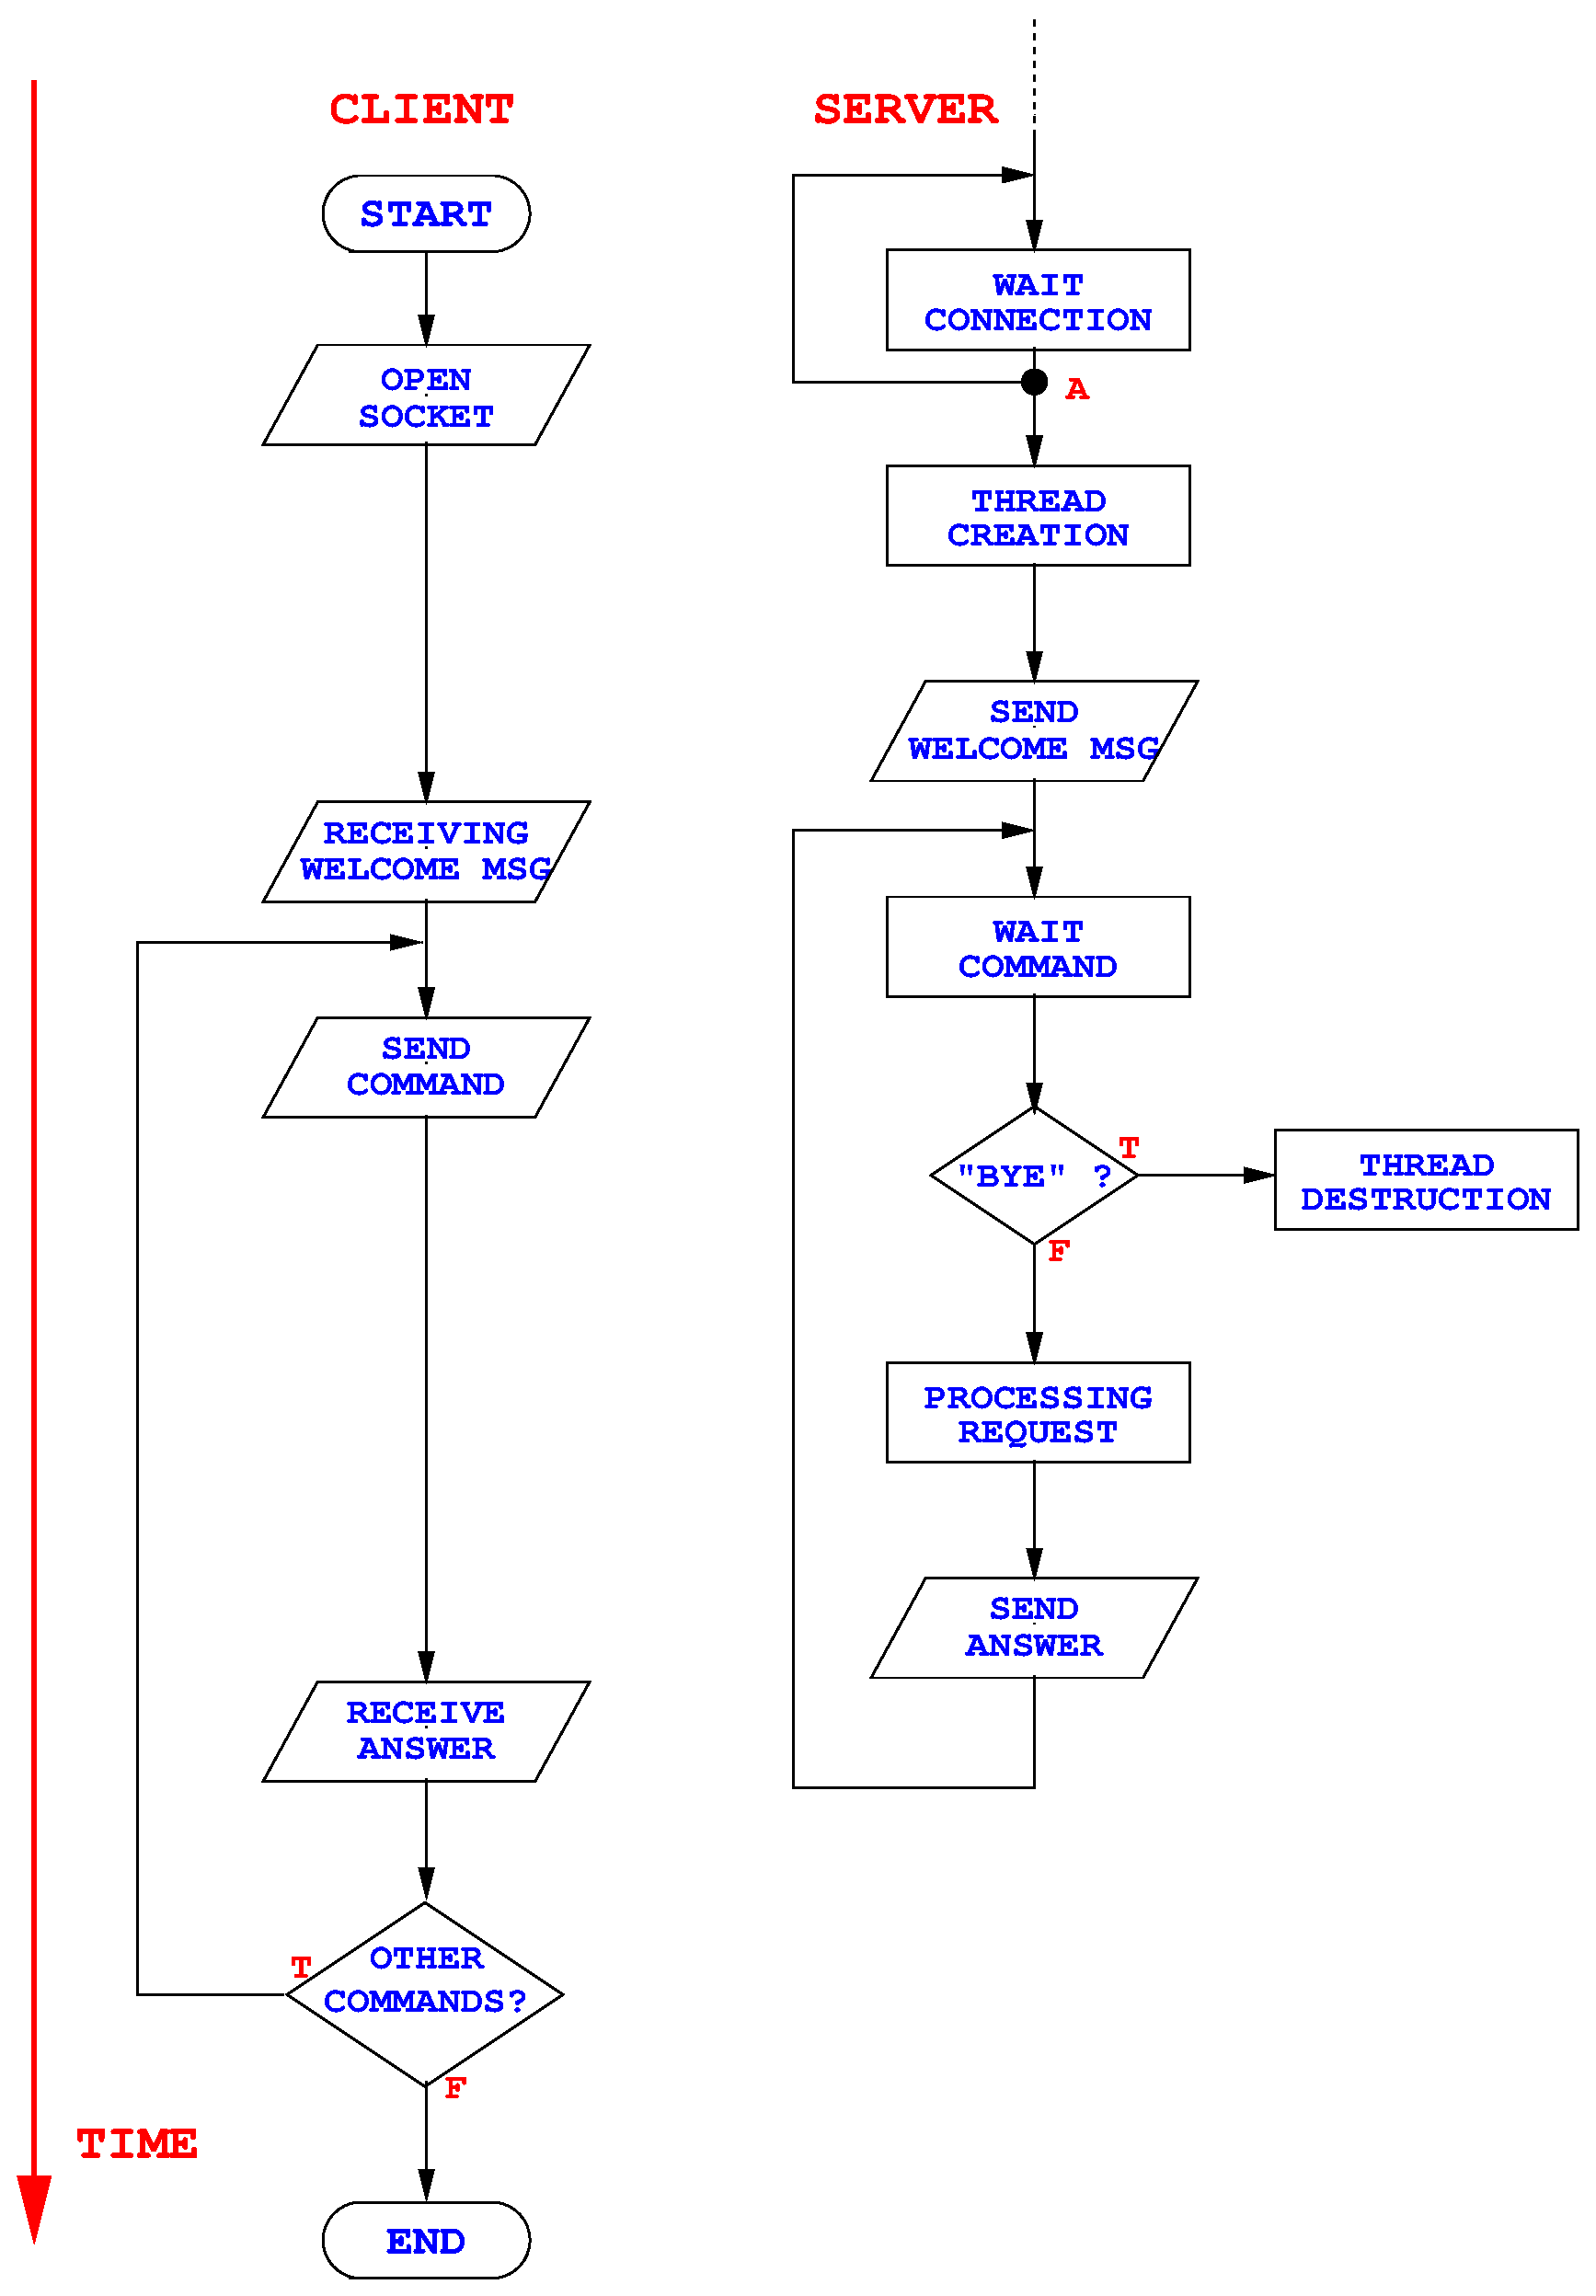
\includegraphics[width=11cm,keepaspectratio]{includes/flow}
\end{center}
\caption{Flow diagram of a typical MCS session}
\label{flow}
\end{figure}
%
The arrow indicates sliding of the time, as we can see different
blocks on client and server aren't contemporaries. Furhermore we see
that while for the client the start and end point are well defined,
for the server we don't have such points because we suppose it is
executed indefinitely. Usually the server waits for a client to open a
TCP socket. When such a socket is opened, the server creates a new
thread of execution and assign the connection to it. We can notice
(point labelled ``A'' in Fig. \ref{flow}), that at this point the
execution path of the server is splitted in two, one of which returns
to wait for another client, while the other start to process client
requests on another thread. Threads are basically identical programs
working on different data. In this case the different data are the
different sockets connected to different client. That's how the server
can process requests from several clients ``simultaneously''.
%
As soon as the new thread is ready, it will send a welcome message
through the socket. Receiving this message indicates that the server
is ready to process client requests, from now on the server will wait
for commands to arrive, while the client will enter a loop to send all
necessary commands and receiving the related answers. When the server
receive a command it will check if it is a \verb|BYE| command, that is
a command to close connection. If it is the thread will destroy
himself. If it isn't the server will process the request and send the
answer until the client sends a \verb|BYE| command.



\section{Accessing a MCS service}
To connect to a \mcs service you should use one of the available
interfaces in the different languages: C, C++, Fortran, IDL or
PHP. One of the main feature of these interfaces is that the syntax
(except for the C++ interface) is quite similar, as will be shown
below. In the following sections we'll assume that the reader has a
minimum knowledge of the object oriented paradigm, as well as the C++
syntax. Furthermore we'll mention some of the \mcs's classes, whose
reference documentation can be found at
\verb|http://spora.ifc.inaf.it/mcs|.


\subsection{User environment}
Once a user has connected and logged in (see Sect. \ref{sec:login}) to
a \mcs service it has a dedicated environment consisting of:
\begin{itemize}
\item a work directory: where the user can upload or download files;
\item a database connection: so that a user can store temporary tables
  that are visible only to the user itself;
\end{itemize}

\noindent In this document we will refer to the work directory on the
server with \verb|CLIPATH|. With the same name we'll refer to the
directory on the client side from which or to which files are uploaded
or downloaded (see Fig. \ref{fig:dirs}). In the same figure you can
see a directory called \verb|SRVPATH| above the \verb|CLIPATH| one,
this is the server main directory which contain all works directories.

%
\begin{figure}[hbtp]
\begin{center}
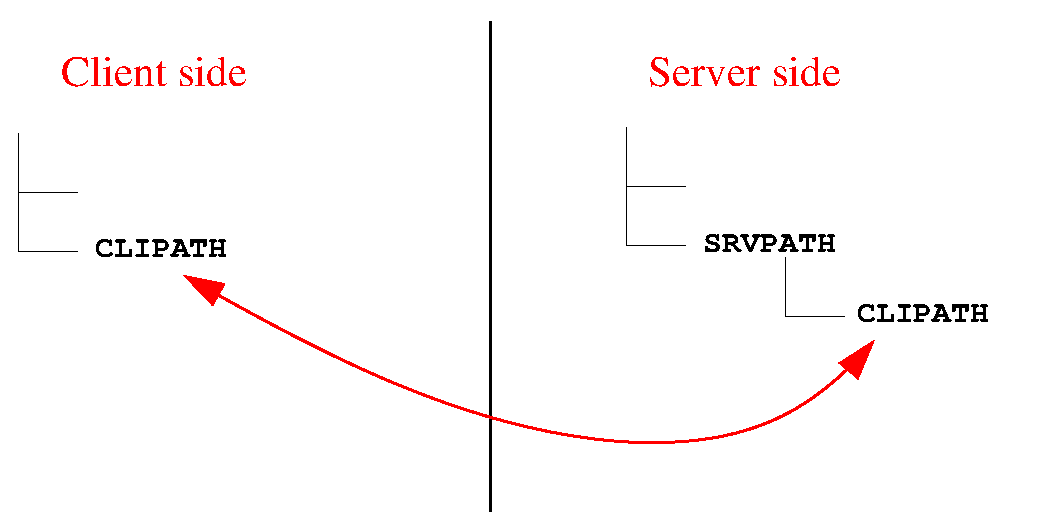
\includegraphics[width=14cm,keepaspectratio]{includes/dirs}
\end{center}
\caption{Directories in a MCS based system}
\label{fig:dirs}
\end{figure}
%



%\noindent The \mcs application server also has a customizable ``local
%directory, inside which are located the work directory for users. In
%the rest of the document we'll refer to this directory with:
%\verb|APPD|, and to the work directory of a user with \verb|WORK|. The
%\verb|APPD| directory can store also a SQL files (list of SQL
%instructions), shell scripts, and batch files (list of \mcs commands),
%which user can execute.



\subsection{Commands}
\label{sec:commands}
Users can request a service from a \mcs based application server using
\textbf{commands}. there are two types of commands: \textbf{base
commands} are those implemented in \mcs itself, \textbf{custom
commands} are those implemented by users (see
Chap. \ref{chap:developer}, ``Developer's manual'').

\noindent A command is a sequence of character terminated by a newline
character, encoded in ASCII. It usually require one or more parameters,
depending on the command itself. The Tab. \ref{tabComandi} shows a
list of available \textbf{base commands}.

\noindent A command can be prefixed by one or more mnemonic switches,
which will modify the execution of the command.

\begin{table}[!ht]
\begin{center}
\caption{MCS Command codes}\label{tabComandi}
\bigskip
\begin{tabular}{|l|l|l|}
  $Switch$&$$&$Meaning$\\
  \hline %
  \hline %
  \verb|ADM| & & Administration command,                \\
  \verb|WRK| & & Search the script in the work directory\\
  \verb|SQR| & & Save query result in a file            \\
  \hline %
  \hline %
  $Command\ code$&$Parameter$&$Meaning$\\
  \hline %
  \hline %
\verb|USR |&\verb|<username>         | &User name                             \\
\verb|PWD |&\verb|<password>         | &Password                              \\
\verb|DBN |&\verb|<DB name>          | &DB name to be used                    \\
\verb|CON |&\verb|                   | &Login                                 \\
\verb|BYE |&\verb|                   | &Closes the connection                 \\
\verb|CID |&\verb|                   | &Asks for the CID (Client Identifier)  \\
\verb|QRY |&\verb|<query>            | &Execute a SQL query                   \\
\verb|ROWS|&\verb|                   | &Asks for the number of returned rows  \\
\verb|FLD |&\verb|                   | &Asks for the number of returned fields\\
\verb|QRES|&\verb|                   | &ROWS, FLD, send query results         \\
\verb|SQL |&\verb|<sql_script> [Pars]| &Execute a SQL script, with parameter  \\
\verb|SCR |&\verb|<script>     [Pars]| &Execute a shell script, with parameter\\
\verb|BAT |&\verb|<bat_script> [Pars]| &Execute a BATCH script, with parameter\\
\verb|GET |&\verb|[<file_name>]      | &Retrieve a file from work directory   \\
\verb|PUT |&\verb|<file_name> <size> | &Send a file to the work directory     \\
\verb|GETDATA |&\verb|               | &Retrieve the next \verb|MyData| object\\
\verb|PUTDATA |&\verb|               | &Send a \verb|MyData| object           \\
  \hline %
  \hline %
\end{tabular}
\end{center}
\end{table}

\subsubsection{Command \tt{USR <username>}}
Used to supply the user name to the applications server during
authentication. The account identify a list of grants.

\bigskip
\verb|usr giorgio|
\bigskip

\subsubsection{Command \tt{PWD <password>}}
Used to supply the password for a specific account.

\bigskip
\verb|pwd my_password|
\bigskip


\subsubsection{Command \tt{DBN <DB name>}}
Used to select the DB on which you wish to operate.

\bigskip
\verb|dbn test|
\bigskip

This way you will acess the database named \verb|test|.


%\subsubsection{Command \tt{DBH <DB server>}}
%Con questo command si indica l'indirizzo del database server che si
%vuole utilizzare. Solitamente il database server si trova nella stessa
%macchina dell'application server per cui non \`e necessario utilizzare
%questo command. Questo command pu\`o essere disabilitato tramite lo
%switch \verb|MCS_HAVE_DBH_CMD|. Il command pu'\o essere utilizzato nella
%seguente maniera:
%
%\bigskip
%\verb|dbh sqlhost|
%\bigskip
%
%Cos\`i si imposta l'accesso al database server \verb|sqlhost|. Si
%ricorda che l'indirizzo deve essere raggiungibile dalla macchina sui
%cui viene eseguito l'application server, non il client.

\subsubsection{Command \tt{CON}}
This command doesn't need any parameter, and it is used to finalize the
authentication process. It must be used after the user name, password and
database name have been set by the preceding commands. If the user log in with
success the following commands will be automatically executed:

\bigskip
\verb|bat auto|

\verb|sql env|
\bigskip


\subsubsection{Command \tt{BYE}}
This command is used to close the connection, this means that the serve will
close the MySQL connection, delete all files int he user work directory,
delete all temporary tables e destroy the thread associated with the
client. These cleanup operation are performed also if the client abruptly
closes the socket, but it's a good practice to issue this command before
closing. This command doesn't need any parameter.


%\subsubsection{Command \tt{DBC}}
%Con questo codice command si chiude la sessione MySQL. Questo codice
%command non accetta parametri. Nota che per eseguire altri comandi \`e
%necessario effettuare nuovamente l'autenticazione, eventualmente anche
%con un altro nome utente.


\subsubsection{Command \tt{CID}}
Every client has a \textbf{Client identifier}, that is a unique number that
identify the associated thread. This command asks for this number, and doesn't
need any parameter.

\subsubsection{Command \tt{QRY <query>}}
With this command users can execute SQL queries directly on the DB server. The
query must follow the command code without any quote. Of course you can use
the quotes inside the query itself. If it is a selection query you can use the
\verb|QRES| command to retrieve the result, otherwise you can use the
\verb|SQR| switch to write the result to a file. For non-select queries this
command will return the number of affected records.

\bigskip
\verb|qry SELECT * FROM table|
\bigskip

\noindent Notice that you don't need to supply the '\verb|;|' at the
end of the query, like you would do with the mysql client.


\subsubsection{Command \tt{ROWS}}
Returns the number of affected or selected rows from the last query. It
doesn't need parameters.

\subsubsection{Command \tt{FLD}}
Returns the field list of the last execution of a query, if it is a
select-like query. It doesn't need parameters.

\subsubsection{Command \tt{QRES}}
This command automatically execute \verb|ROWS| and \verb|FLD| in sequence,
then send the result of a query. It doesn't need parameters.

%\subsubsection{Commands \tt{SQL}, \tt{SCR}, \tt{BAT}}
%With these commands it is possible to execute a list of commands (respectively
%in SQL, Shell script, \mcs commands), stored in a file on the application
%server's tree.
%
%Tramite questi codici command \`e possibile eseguire alcune sequenze
%di istruzioni (rispettivamente SQL, Shell script, \mcs)
%memorizzate su un file. Tali script sono parametrizzati in maniera da
%rendere generica la funzionalit\`a offerta. L'esecuzione di questi
%codici command prevede una risposta composta da almeno due
%\textbf{risposte}, indicanti rispettivamente l'inizio e la fine della
%elaborazione. Tra le due \textbf{risposte} di inizio e fine potrebbero
%essere inviate altre \textbf{risposte} (ovvero le risposte ai singoli
%comandi).  Se tra l'inizio e la fine dell'esecuzione avviene un errore
%esso verr\'a segnalato nel modo che compete al command che lo ha
%generato, e l'esecuzione verr\`a bloccata. Anche in caso di errore
%verr\'a comunque trasmessa la \textbf{risposta} finale. Nota che i
%nomi degli script non possono contenere il carattere \verb|'/'| per
%motivi di sicurezza.


\subsubsection{Command \tt{SCR <script> [PARS]}}
This command execute a shell script present in the \verb|APPD/usr/scr| or
\verb|APPD/adm/scr| path (depending if you used the \verb|ADM| switch). An
example of the syntax is:

\bigskip
\verb|scr dqry 'T001.T001' '' '10' '1000'|
\bigskip

This command execute the system command:

\bigskip
\verb|APPD/usr/src/dquery 'T001.T001' '' '10' '1000'|
\bigskip

and writes the standard output on \verb|WORK/out|, and standard
error on \verb|WORK/err|. The \mcs server also replies with the exit code of
the script, so that the user can see if there was any error. The files
\verb|WORK/out| and \verb|WORK/err| can be retrieved with the \verb|GET|
command, otherwise thay can be used for another command with the \verb|WRK|
switch.

\subsubsection{Command \tt{SQL <script> [PARS]}}
This command execute a sequence of SQL instructions, stored in a file in the
\verb|APPD/usr/sql| or \verb|APPD/adm/sql| path (depending if you used the
\verb|ADM| switch). An example of the syntax is:

\bigskip
\verb|sql getrawtable T001|
\bigskip

With this command you execute the SQL script \verb|getrawtable|, passing as
first parameter the string \verb|T001|. If the last query of the script is a
select-like query, then the result can be retrieved with the \verb|QRES|
command.


\subsubsection{Command \tt{BAT <script> [PARS]}}
This command execute a sequence of \mcs commans, just like these we are
dealing with, tored in a file in the
\verb|APPD/usr/scr| or \verb|APPD/adm/scr| (depending if you used the
\verb|ADM| switch). An example of the syntax is:

\bigskip
\verb|bat auto|
\bigskip

Like with the \verb|SQL| command, we can also use parameter for the batch
file.


\subsubsection{Command \tt{GET [<file\_name>]}}
With this command a user can retrieve a file located in the work directory on
the server. The parameter is the file name, if no parameter is passed the file
\verb|WORK/out| will be retrieved. The file will be sent in binary mode.

\subsubsection{Command \tt{PUT <file\_name> <size>}}
With this command a user can store a file in the work directory on the server.
Parameters are the file name and the file size in byte. The file will be sent
in binary mode.

%\subsubsection{Command \tt{SYS <command>}}
%Con questo command \`e possibile eseguire un command di sistema sul
%computer su cui \`e in esecuzione l'application server. Questo command
%pu\`o essere disabilitato tramite lo switch \verb|MCS_HAVE_SYS_CMD|.


\subsection{Login}\label{sec:login}
Commands described above (excluding \verb|USR, PWD, DBN, DBH, CON, BYE|) can
be executed only after the user has logged in. The authentication process
require that you specify the user name, the password and the name of the
database, finally you should send the command \verb|CON| to finalize the
process.


%potranno essere utilizzati
%soltanto dopo la fase di autenticazione, pertanto questi devono essere
%i primi comandi eseguiti. La fase di autenticazione prevede che
%vengano specificati almeno user name, password e nome del database,
%quindi che si dia il command \verb|CON|. Se l'autenticazione va a buon
%fine vengono caricati i permessi dell'utente dalla tabella
%\verb|grants|, quindi vengono automaticamente eseguiti i seguenti
%comandi:
%
%\bigskip
%\verb|bat auto|
%
%\verb|sql env|
%\bigskip\newline
%%
%al fine di inizializzare l'ambiente MySQL.


\subsection{Grants}
When a user access the service it has a list of grants that allow or deny
certain operations. If the \verb|read_grants| is set to zero then all users
have all grants, otherwise grants can be specified on a table named
\verb|grants|. Possible grants are:
\begin{table}[!htb] \begin{center}
    \caption{User's grants}\label{tab:grants1}
    \bigskip\bigskip
    \begin{tabular}{|l|l|}
      \hline
      \textbf{Symbol} & \textbf{Meaning} \\
      \hline
      \verb|MG_NO_GRANTS  | &    no grants       \\
      \verb|MG_LOGIN      | &    login allowed   \\
      \verb|MG_SQL_SCRIPTS| &    command SQL	 \\
      \verb|MG_SCRIPTS    | &    command SCR	 \\
      \verb|MG_QUERY      | &    command QRY	 \\
      \verb|MG_BATCH      | &    command BAT	 \\
      \verb|MG_GET        | &    command GET	 \\
      \verb|MG_PUT        | &    command PUT	 \\
      \verb|MG_SYS        | &    command SYS	 \\
      \verb|MG_ADMIN      | &    command ADM	 \\
      \verb|MG_ALL        | &    all grants above\\
      \hline
    \end{tabular}
\end{center} \end{table}


%\subsection{Funzionalit\`a dell'interprete dei comandi}
%L'interprete dei comandi \mcs ha molti aspetti in comune con una
%classica shell. Esso infatti dispone di comandi mnemonici con
%eventuali parametri separati da spazio, ed i risultati vengono inviati
%in chiaro come se si trattasse di uno standard output. Inoltre il
%client deve sempre aspettare il prompt prima di impartire un nuovo
%command. L'utente dispone anche di una propria work directory in cui
%pu\`o memorizzare file temporanei e trasferirli attraverso la
%rete. Per i dettagli sul protocollo di comunicazione vedi il capitolo
%dedicato. Diamo qui una breve panoramica sulle funzionalit\`a offerte
%dall'interprete dei comandi: un command \mcs \`e composto da tre parti
%separate da spazi: switch (opzionale), codice command, parametri
%(opzionali). Segue una breve descrizione degli switch:
%
%\begin{enumerate}
%\item  \verb|WRK|: se usato il percorso per la ricerca degli
%  script verr\`a sostituito con la work directory dell'utente;
%\item \verb|SQR|: se usato con un command che effettua una query di
%  selezione, il risultato verr\`a scritto su un file nella work
%  directory;
%\item \verb|ADM|: indica che il command che segue \`e un command di
%  amministrazione, ci\`o significa che la ricerca degli script verr\`a
%  eseguita nella directory degli script di amministrazione. Il command
%  verr\`a eseguito solo se l'utente ha i diritti di amministrazione;
%\end{enumerate}
%
%Di seguito sono elencati alcuni comandi ed il loro utilizzo:
%\begin{enumerate}
%\item \verb|QRY|: esegue una query SQL sul database;
%\item \verb|SCR|: esegue uno script sul�server, scrivendo il
%  risultato su un file nella work directory;
%\item \verb|GET|: permette di trasferire un file presente nella work
%  directory;
%\item \verb|QRES|: permette di trasferire il risultato di una query;
%\item \verb|SQL|: esegue uno script SQL memorizzato sul server, con
%  sostituzione di parametri;
%\item \verb|BAT|: esegue un file batch di comandi
%\end{enumerate}

Per accedere al servizio l'utente deve innanzitutto aprire un socket
TCP, quindi effettuare la fase di autenticazione (vedi
Sez. \ref{sec:login}). A questo punto si possono eseguire i comandi
\mcs o quelli supportati dall'applicazione creata. Per eseguire un
command bisogna aspettare il prompt (\verb|#0--|), quindi inviare il
command come descritto precedentemente. Il server replicher\`a con una
o pi\`u stringhe di risposta, eventualmente passando in modalit\`a
dati, fino ad inviare il successivo prompt. Per chiudere la sessione
\`e possibile chiudere il socket oppure inviare il command
\verb|BYE|. Bisogna tener presente che il server \mcs prevede un
periodo di inattivit\`a massima di 30 minuti, dopodich\`e la
connessione viene chiusa automaticamente (da implementare).




\chapter{Interface to MCS}
While it is possible to access a \mcs system from a simple telnet client, only
a more sophicated program can take advantage of all \mcs's feature. So we
developed a C++ class that simplify access to \mcs services, its name is
\verb|mcscli|.

\noindent Furthermore we developed a system of C macros, named \textbf{IFD}
(Interface Descriptor), capable of generate code for a C wrapper to a C++
library, and translate a C++ interface to a meta-language. We used
\textbf{IFD} with the following classes of the \mcs library:
\begin{itemize}
\item \verb|MyData|
\item \verb|MyVector|
\item \verb|DBFac|
\item \verb|mcscli|
\end{itemize}
So we have a C wrapper to these classes (its interface is in the file
\verb|mcs_c.h|, and the object code is compiled into the \mcs library).

\noindent Other languages can also use \mcs classes through some
interface. Actually we developed an interface to the following languages:
\begin{itemize}
\item \textbf{PHP}: the interface relies upon the C wrapper, and it is
  automatically generated by a program named \textbf{SWIG}
  \footnote{www.swig.org};
\item \textbf{IDL}: the interface relies upon the C wrapper, and it is
  generated using the meta-language produced by \textbf{IFD} and a perl
  program named \verb|c2idl|.
\end{itemize}

\noindent Subject of this chapter are the description of all these interfaces
and their usage.


\section{The mcscli class}
(TO BE WRITTEN)


%\section{The Interface Descriptor (IFD)}
%(TO BE WRITTEN)
%
%The \textbf{IFD} is basically a set of C macros contained in the file
%\verb|ifd.h|, installed with \mcs. Its main purposes are to generate a
%C wrapper to some C++ classes, and a meta-language which describes these
%classes. To use \textbf{IFD} you must create an header file which contain the
%description of your C++ code. This description is made using the \textbf{IFD}
%macros as shown in the following files installed with \mcs:
%\begin{itemize}
%\item \verb|MyData_c.h|: description of the interface to class \verb|MyData|;
%\item \verb|MyVector_c.h|: description of the interface to class
%  \verb|MyVector|;
%\item \verb|DBFac_c.h|: description of the interface to class \verb|DBFac|;
%\item \verb|mcscli_c.h|: description of the interface to class \verb|mcscli|;
%\item \verb|mcs_c.h|: includes header needed by the C wrapper, and all the
%  above files.
%\end{itemize}
%
%\noindent The interface should contain all constructors and destructor of the
%classes you wish to use.
%
%Macros which describes the interface are the following:
%\begin{itemize}
%\item \verb|IFD_CONSTRUCTOR(CLASS, CPARS)|: to describe a class constructor,
%  its parameters are the name of the class
%							
%IFD_COPY_CONSTRUCTOR(CLASS)
%							
%IFD_DESTRUCTOR(CLASS)
%
%IFD_WRAP(RETTYPE, CLASS, METHOD, CALL)
%
%IFD_WRAP_VOID(CLASS, METHOD, CALL)
%
%IFD_C_WRAP(RETTYPE, FUNCTION, CALL)
%
%IFD_C_WRAP_VOID(FUNCTION, CALL)
%\end{itemize}


\section{Interface usage and naming convention}
In this section we describe how to use the interfaces, and the naming
convention used. These information are valid for all interfaces, see the
following sections for information related to a specific interface.

\noindent Actually the following \mcs classes are availables in all
interfaces:
\begin{itemize}
\item \verb|MyData|
\item \verb|MyVector|
\item \verb|DBFac|
\item \verb|mcscli|
\end{itemize}
For a detailed description of all these classes and their methods check the
relative documentation. Note that not all members are wrapped, that's because
C cannot handle overloaded functions. Check the classes documentation to see
if a method is wrapped or not.

\noindent Before using a class you must call the appropriate wrapper to the
constructor which returns the memory address where the object has been
allocated. You should not modify this address, neither modify the type of the
variable where the address has been stored (for those languages that let you
do this), otherwise the object will become unreachable. We recommend to
destroy objects when they are no longer needed, you can do this by calling the
appropriate wrapper to destructor and passing the address of the object to be
destroyed. The memory address must also be passed to all those wrappers to
methods of that class.

\noindent \textbf{Important note:} What is returned by the wrapper to
constructor routine is just a memory address, so the language you are using
(even C!)  doesn't know anything about the type of object that has been
created. For this reason, if you use this address with a wrapper of another
class, your compiler won't give you any error message. Furthermore your
program will probably die because of a segmentation fault.


\subsection{Error handling}
\label{ssec-Error handling}
Many \mcs class uses exceptions to handle errors, but this mechanism is not
available in C, nor in other languages for which we have an interface. Because
we don't wanted to use the ``C-Style'' error handling, that is checking the
return value of a function after each call to see if an error occurred, we
implemented another mechanism very similar to the one used in the
\verb|CFITSIO| library:

\noindent Any routine require an extra parameter, named \verb|STATUS|, that is
an address to a \verb|ifd_status| structure (defined in \verb|ifd.h|) which
contains a flag that tells if an error occurred in a previous call. This flag
will be checked everytime a routine is called, and if it is set, the routine
will return immediately. If the flag is not set the routine will perform its
task, and if it generates an error it will set the flag and write an error
messages in another field of the structure.

\noindent This way you can, if you use always the same \verb|ifd_status|
structure, check if an error occurred only at the very end of a sequence. The
Sect. \ref{ssec-Routines provided by IFD} shows how to allocate, free, and
manipulate a \verb|ifd_status| structure.

\noindent In the following sections we'll explain the naming convention for a
generic class named \verb|CLASS|. Arguments in brackets (\verb|<>|) are
specific to a function or method. Arguments named \verb|addr| are the the
memory address of an object, those named \verb|status| are the status variable
used in error handling.

\subsection{Constructors}
\label{ssec-Constructors}
Constructors follows this name convention:
\begin{verbatim}
  addr = new_CLASS(<PARAMETERS>, status)
\end{verbatim}
where the parameters are the ones needed by the constructor. Note that only
one constructor can be wrapped so check the documentation to check wich one is
used. These functions returns the memory address where the object has been
allocated. You must use this address in the subsequent method calls. In all
interfaces this memory address is stored in a numeric variable, you should
avoid changing its value or type of the variable.

\subsection{Destructors}
\label{ssec-Destructors}
Destructors follows this name convention:
\begin{verbatim}
  del_CLASS(addr, status)
\end{verbatim}
These functions doesn't need any specific parameter, but only the address of
the object to be destroyed, and the status variable. Note that you should call
the appropriate destructor (the one belonging to the same class with which the
object was created), otherwise you will surely get a segmentation fault.
These functions doesn't return any value.

\subsection{Copy constructors}
Copy constructors follows this name convention:
\begin{verbatim}
  newaddr = copy_CLASS(addr, status)
\end{verbatim}
These functions doesn't need any specific parameter, but only the address of
the object to be copied, and the status variable. Note that you should call
the appropriate copy constructor (the one belonging to the same class with
which the object was created), otherwise you will surely get a segmentation
fault. These functions returns the memory address of the newly created
object.

\noindent \textbf{Note:} actually only the \verb|MyData| class has a copy
constructor, because it is the only one for which it makes sense.

\subsection{Methods}
\label{ssec-Methods}
Methods follows this name convention:
\begin{verbatim}
  retval = CLASS_methodname(addr, <PARAMETERS>, status)
\end{verbatim}
where the parameters are the ones needed by the method. Note that there can be
only one method with a certain name, because overloading is not supported. The
type and meaning of the return values depend on the method called, check the
class documentation.

\subsection{Routines provided by IFD}
\label{ssec-Routines provided by IFD}
In this section we'll examine some facilities provided by the \verb|ifd|
system to handle the ``status'' variables. All of these routines (except
\verb|ifd_null|) requires a ``status'' variable as parameter.
\begin{enumerate}
\item \verb|status = ifd_new_status()|: this function will creates a new
  ``status'' variable and return its memory address. These memory address will
  be used in subsequent call to the routines of the \mcs interfaces;
\item \verb|ifd_del_status(status)|: this function will destroy a ``status''
  variable previously created with \verb|ifd_new_status|, it doesn't return
  any value;
\item \verb|str = ifd_last_error(status)|: this function will return the error
  messages generated by the last error, if any, otherwise an empty string is
  returned;
\item \verb|ii = ifd_got_error(status)|: this function will return an integer
  value of 0 if no error has occurred, 1 otherwise. Note that if an error
  occurred subsequent call to the \mcs interfaces with the same ``status''
  variable will do nothing. At this point you can end your job or call
  \verb|ifd_reset_error| to reset the error flag and continue.
\item \verb|ifd_reset_error(status)|: this function will reset the error flag
  of the ``status'' variable passed as paramter. It doesn't return any value;
\item \verb|ii = ifd_null()|: some functions of the \mcs interface require a
  pointer to null, that is simply an unsigned integer (4 bytes long) with a
  value of zero. For some languages giving this variable as parameter is not
  immediate, so we provide this function that return the correct null pointer
  for your language. It doesn't need any parameter;
\end{enumerate}

\section{The C interface}
\label{sec-The C interface}
The header file for the C interface is \verb|mcs_c.h| and it is located in the
\mcs include directory, while the code is built inside the \mcs library. So
you can compile and link you program as you would do with any other \mcs based
program:
\begin{verbatim}
  cc `mcs-config --cflags` -c myprog.c
  cc -o myprog myprog.o `mcs-config --libs`
\end{verbatim}

\noindent There is an example on how to use the C inteface in
\verb|prefix/share/mcs/share/test/c_test.c|. You can compile this program
typing \verb|make| in the test directory.


\section{The PHP interface}
\label{sec-The PHP interface}
The PHP nterface should be build before it can be used. To do this, after \mcs
has been installed, switch to user \verb|root| and change to the directory
\verb|prefix/share/mcs/client/php|.  Here you will find a \verb|Makefile| in
which you can modify the variables in the ``user customizable section'' to fit
your system's settings. Actually this section contains only the path to the
include directory of PHP.  When you're done with
the settings you can issue the command \verb|make| to build the interface in a
shared library named \verb|php_mcs.so|. In the same directory you will
find a file named \verb|mcs.php| which contains the code that will load the
shared library, copy this file in the directory where your PHP code will run,
then edit to specify the path of the library (that is locate the string
``php\_mcs.so'' and substitute with
``prefix/share/mcs/client/php/php\_mcs.so''). Furthermore you will find a
file named \verb|testphp.php4| which you can use to test the interface
functionality and as a starting point to write other programs.

\noindent To test the PHP interface copy the files \verb|testphp.php4| and
\verb|mcs.php| in a temporary directory, modify the latter as described above,
then type the following command:
\begin{verbatim}
  php testphp.php4
\end{verbatim}




\section{The IDL interface}
\label{sec-The IDL interface}
The IDL interface should be build before it can be used. To do this, after
\mcs has been installed, switch to user \verb|root| and change to the
directory \verb|prefix/share/mcs/client/idl|. Here you will find a
\verb|Makefile| in which you can modify the variables in the ``user
customizable section'' to fit your system's settings. Actually this section
contains only the path to the include directory of IDL. When you're done with
the settings you can issue the command \verb|make| to build the interface in a
shared library named \verb|widl_libmcs.so|. In the same directory you will
find a file named \verb|widl_libmcs.pro| which you can place in the directory
where you store your \verb|.pro| files for IDL. Furthermore you will find a
file named \verb|testlibmcs.pro| which you can use to test the interface
functionality and as a starting point to write other programs.

\noindent To test the IDL interface copy the file \verb|testlibmcs.pro| in the
directory where you store your \verb|.pro| files and type the following
commands in a IDL prompt:
\begin{verbatim}
  .r widl_libmcs
  .r testlibmcs
  testlibmcs
\end{verbatim}


%---------------------------------------------------------------------
\chapter{Developer's manual}
\label{chap:developer}

\section{Communication protocol}
The communication protocol is the set of technical rules that drives
the information exchange between the client and the server. To make
the system works it is necessary that both parts implements rigorously
these rules. A detailed description follows.

\subsection{The socket}
The communication between the client and server relies on a
bidirectional stream, called TCP socket, which is platform
independent, so a user can connect from any platform and any operative
system. The only requirement is that the client program can read and
write using the ASCII character set, and optionally in binary.

\subsection{Working modes}
\mcs can work in two distinct working modes:
\begin{itemize}
\item \textbf{Control mode:} in this mode client and server
  exchange mnemonic strings in the ASCII character set, called
  \textbf{Control strings}. More specifically these strings are called
  \textbf{Commands} if sent from the clients, \textbf{Answers} if sent
  from the server. The \textbf{Control strings} have a special syntax
  based on delimitators;

\item \textbf{Data mode:} this mode is used to send data across the
  network. Data can travel only in one direction, so we have a data
  mode \textbf{towards} the server (subsequent to a \verb|PUT|
  command), or \textbf{towards} the client (subsequent to a \verb|GET|
  command). Some \textbf{Control strings} are provided to inform the
  client that the server is changing \textbf{working mode};
\end{itemize}

\subsection{Syntax in control mode: commands}
\textbf{Commands} are strings of ASCII characters sent from the client
to request a service from the application server. The detailed syntax
follows:

\begin{itemize}
\item \textbf{Switch (optional):} this string is made up of one or
  more alfanumeric character (exluding whitespace characters) and it
  is used to modify the behaviour of the server for the associated
  command;
\item \textbf{Separator:} a blank or tab character. If there isn't any
  switch in the command this field should not be transmited;
\item \textbf{Command code:} this string is made up of one or more
  alfanumeric character (exluding whitespace characters), and it is
  used to specify which request the client is asking for. Some command
  codes requires parameters;
\item \textbf{Separator:} a blank or tab character. If the command
  code doesn't requires parameters this field should not be
  transmitted;
\item \textbf{Parameters:} number, meaning and
  syntax of parameters depends on the command. If the command code
  doesn't requires parameters this field should not be transmitted;
\item \textbf{EOC, End of Command:} a newline character (ASCII code 10, base
  10). The server will start to process the request after receiving of this
  character;
\end{itemize}
%
\textbf{Command codes} and \textbf{switches} are case insensitive,
\textbf{parameters} may not be. As an example consider the following command:

\bigskip
\verb|sqr qry select * from tfields\n|
\bigskip

$\underbrace{\textbf{sqr}}_{switch}\underbrace{\textbf{\ }}_{bl}$
$\underbrace{\textbf{qry}}_{code}\underbrace{\textbf{\ }}_{bl}$
$\underbrace{\textbf{select * from tfields}}_{parameter}$
$\underbrace{\textbf{\textbackslash n}}_{EOC}$
\bigskip \newline
%
This commands request the execution of a SQL query on the
database. The \verb|SCR| switch tells \mcs to save the result in
a file in the work directory. For a complete list of
\verb|command codes| and relative parameters see Tab.
\ref{tabComandi}.

\subsection{Syntax in control mode: answers}
\textbf{Answers} are strings of ASCII characters sent from the server
in reply to a \textbf{command}. The message contained in the
\textbf{answers} is presented in both codified and descriptive
form. The syntax description follows:
\begin{itemize}
\item \textbf{BOA, Beginning of Answer:} the character '\verb|#|'
  (hash) states that a new \textbf{answer} is beginning;
\item \textbf{Answer code:} it is made up of three digits, and
  represent the codified form of \textbf{answer}. In particular, if
  the first digit is zero then the command was executed successfully,
  otherwise an error or warning occurred. The least two digits gives
  more details;
\item \textbf{Description:} is a human readable description of the numeric code;
\item \textbf{EOA, End of Answer:} a newline character (ASCII code 10, base
  10), it is used to notify the user that the answer is completed.
\end{itemize}
%
Consider the following example:

\bigskip

\begin{verbatim}
#001Welcome at glinux.local running ...\n
\end{verbatim}
\bigskip

$\underbrace{\textbf{\#001}}_{BOA + code}$
$\underbrace{\textbf{Welcome at glinux.local running ...}}_{Description}$
$\underbrace{\textbf{\textbackslash n}}_{EOA}$
\bigskip \newline
%
It is the welcome message of the \mcs server. Some
\textbf{answers} contains an auxiliary numeric field between the
\textbf{answer code} and the \textbf{description}, as showed by the
following example, that is the \textbf{answer} to the \textbf{command}
\verb|CID| which asks the server for the client identifier (see
Tab. \ref{tabComandi}):

\bigskip
\verb!#015|7|(Client ID)\n!

\bigskip
$\underbrace{\textbf{\#015}}_{BOA + code}$
$\underbrace{\textbf{\textbar}}_{Sep.}$
$\underbrace{\textbf{7}}_{Aux.\ field}$
$\underbrace{\textbf{\textbar}}_{Sep.}$
$\underbrace{\textbf{(Client ID)}}_{Description}$
$\underbrace{\textbf{\textbackslash n}}_{EOA}$
\bigskip \newline
%
Once the client has sent the \textbf{command} must wait for at least
one \textbf{answer}. Then it must check for the presence of the hash
and the first digit of the code, to verify that the command were
executed successfully. Subsequently it can use the rest of the
\textbf{answer}. For certain \textbf{commands} the server could reply
with more than one \textbf{answer}, and possibly it would change to
\textbf{data mode}, so the client must wait for the next prompt before
issuing a new command. The prompt has the following syntax:

\bigskip
\verb!#0--\n!

\bigskip
$\underbrace{\textbf{\#0- -}}_{BOA + prompt}$
$\underbrace{\textbf{\textbackslash n}}_{EOA}$
\bigskip \newline
%
Notice that the first prompt is sent just after the welcome message.



\subsection{Data mode}
The \textbf{data mode} is used to exchange binary data between the
client and the server, in both directions. We will distinguish the
direction on which the data is transmitted:

\subsubsection{Towards the client}
When the server toggle to \textbf{data mode} to send data to client it
uses one of the following \textbf{answers}:

\begin{verbatim}
#009Sending binary data:|1024| bytes.
#010Sending binary file |filename| : |1024| bytes.
#012Sending chunk |1024| bytes.
#028Sending fields details |10|
\end{verbatim}
%
The auxiliary field in the first three tells how many bytes the server
is going to send. So the client must read exactly the same number of
bytes from the socket after the \textbf{EOA} have been read. The
second form gives also the name of the file that is going to be
sent. A very important note on the second form is that the data stream
will not be sent after this \textbf{answer}, but instead will be
splitted in chunk and sent using the third form. The fourth form is
used when the server is going to send the result of a query, it will
gives the name of the fields separated by newline. In this case the
client must read 10 field names separated by newlines. After any of
these \textbf{answers} and the stream of data has been sent the server
will toggle back to \textbf{control mode} and send the following
\textbf{answer}:

\begin{verbatim}
#013End of binary data.
\end{verbatim}


\subsubsection{Towards the server}
It is possible to send binary data towards the server using the
\verb|PUT| command, with which the client can store a file in the
work directory of the server. For further details see the description
of the command \verb|PUT| later.



\chapter{Examples}
\label{chap:examples}
\end{document}
